% 
%jff-notes
%
\documentclass[10pt]{article}
\usepackage[pdftex]{graphicx}
\usepackage{amssymb}
\usepackage{latexsym}
%\usepackage{relsize}
\usepackage{textcomp}
%processed for 10 pt 
%\documentstyle[epsf,psfig]{article}
%\documentstyle[epsf]{article}
\oddsidemargin 0pt
\topmargin -0.0cm
\textwidth 6.2in
\textheight 8.5in
\baselineskip 18pt
%\renewcommand{\baselinestretch} {1.5}
\newenvironment{nitemize}
   {\begin{list}{\begin{math}\bullet\end{math}}%
      {\setlength{\leftmargin}{5mm}
       \setlength{\topsep}{1mm}
       \setlength{\parsep}{0in}
       \setlength{\itemsep}{.7mm}}}%
   {\end{list}}

\newcommand{\fract}[2]{\frac{\textstyle #1}{\textstyle #2}}
\newcommand{\trans}[3]{#1 \stackrel{#2}{\longrightarrow} #3}
\newcommand{\notrans}[3]{#1 \stackrel{#2}{\not\! \longrightarrow} #3}
\bibliographystyle{plain}
\begin{document}
\title{An experimental plugin for decoding CW\\
{\small user's guide {\footnote {\copyright J van Katwijk}}\\
Revised edition of the plugin}}
\author{
Jan van Katwijk\\
Lazy Chair Computing \\
The Netherlands\\
{\em J.vanKatwijk@gmail.com}}
%\date{}
\maketitle
%\baselineskip 22pt
\ \\
\ \\
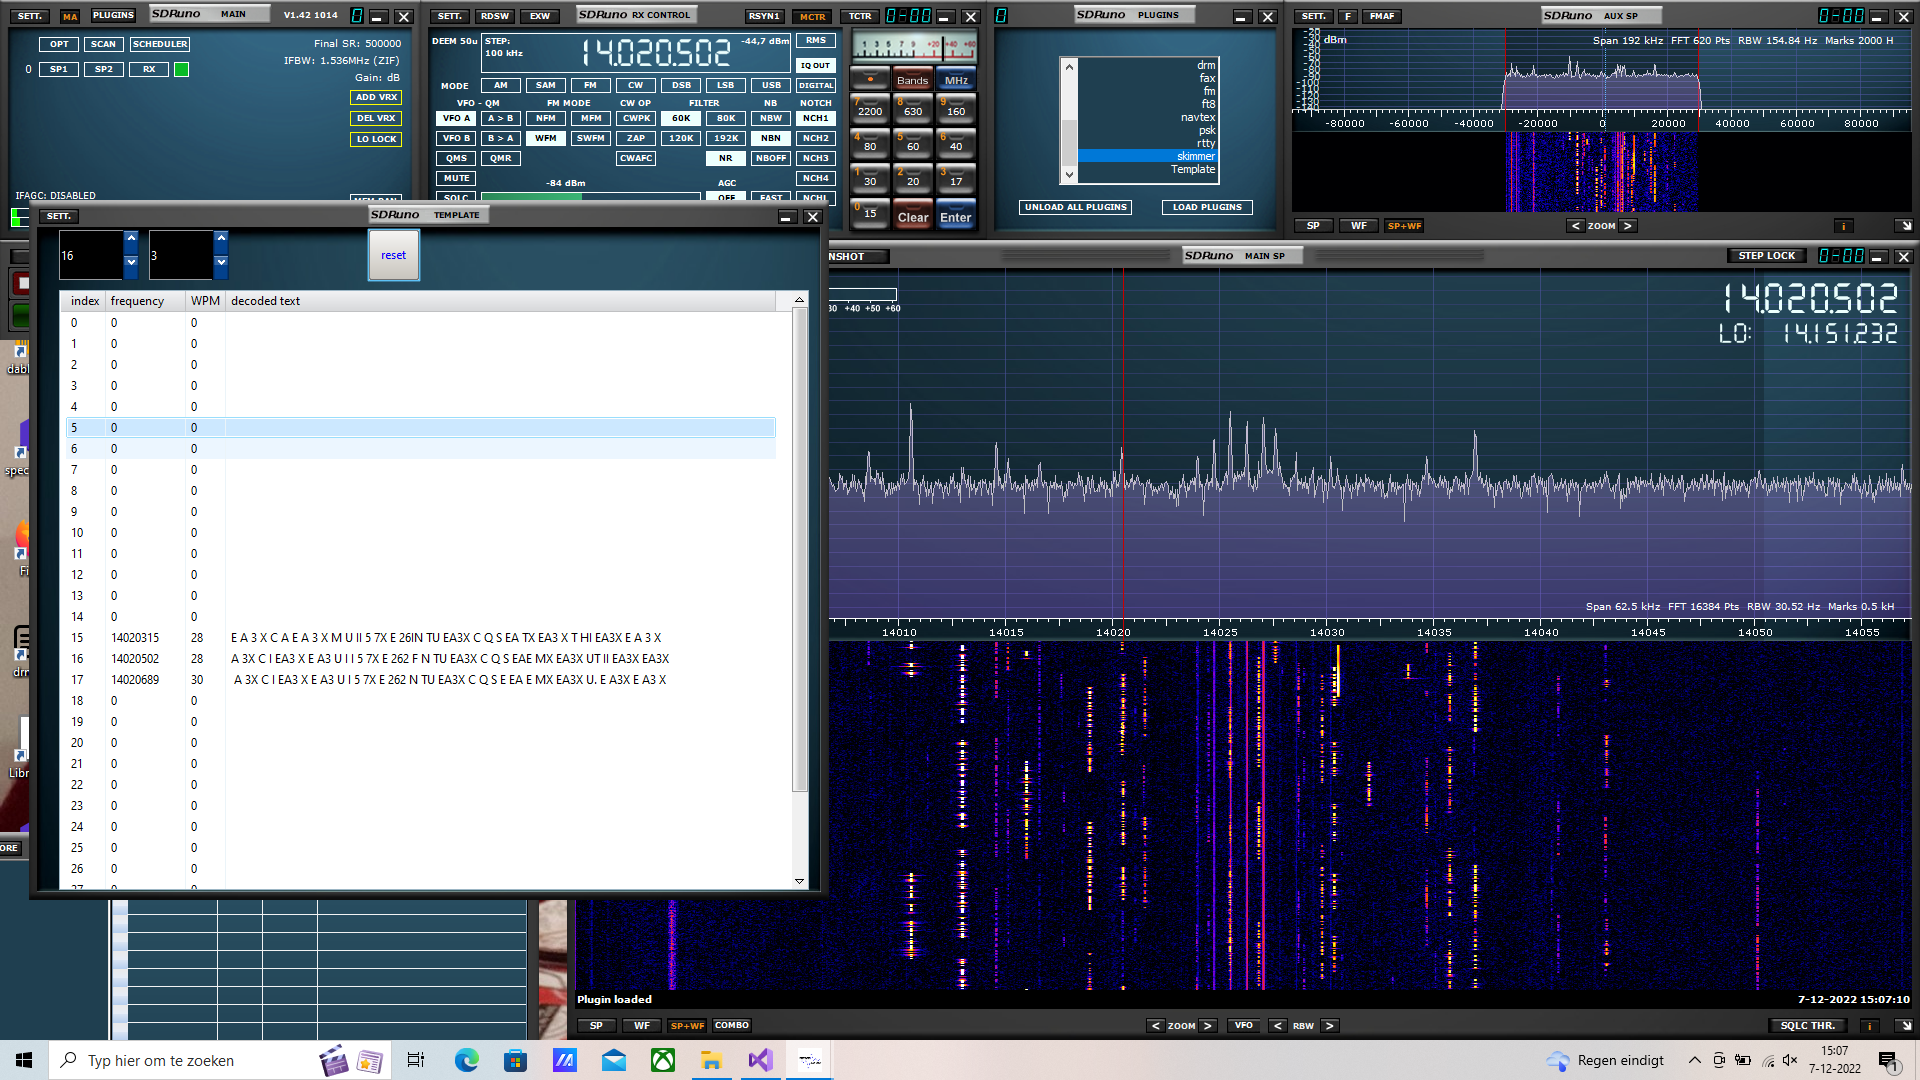
\includegraphics[width=160mm]{skimmer.png}
\ \\
\section{Background}
The biggest problem I have when using the CW decoder plugin is tuning. 
After all, tuning shoud be very accurate and manually tuning is not
easy with all the flickerings on the screen of signals "of" and "off"
\par
While the CW decoder plugin provided some support for tuning correction,
I was not very happy with it.
\par
Therefore a completely different approach was taken in this "skimmer" type
plugin.
Basically it is simple, the incoming samples, rate 192000, are per segment of
2 milliseconds, i.e. 2 * 192 samples, fed into an FFT processor with 
2048 "bin"s.
Each bin then shows the "energy" of the signal in a frequency band with
a width of 192000 / 2048, i.e. slightly less than 100 Hz.
\par
Then from some specified bins the data is sent to a decoder, 
the samplerate of that data is then obviously app 500 samples a second.
Note that a 30 WPM signal takes app 40 mseconds per dot, so that is covered
by app 20 samples.
\par
This plugin provides means for decoding the signal from a group of successive
bins.
\section{The plugin}
The plugin itself is straightforward, and contains a top line with two
selectors and a button, and a field with 32 lines.
The area of interest is a region of 32 bins (i.e. about 3 Khz)
around the selected frequency.
\par
Each line contains 4 elements
\begin{itemize}
\item a line number, i.e. one in the range of 1 .. 32;
\item a frequency indicator. If data in the bin is decoded, the
frequency indicator gives the precise frequency for the data in that bin;
\item a WPM indicator. If data in the bin is decoded, the
WPM indicator gives an estimate of the Words per Minute of the decoded data;
\item the text, the last 85 characters of the text.
\end{itemize}
The indicators tell which bins are selected for data decoding:
\begin{itemize}
\item the right selector, with as default value 3, tells how many bins
are selected for decoding the data (always an odd number);
\item the left selector, with as default value 6, tells the line number
of the bin that is central in the selected bins.
\end{itemize}
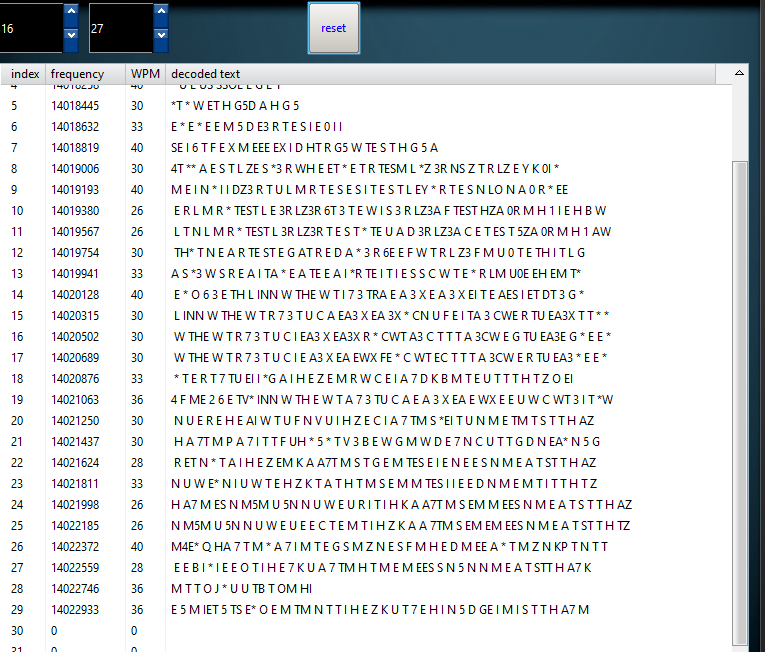
\includegraphics[width=60mm]{skimmer-2.png}
\section{Copyright}
The code for this plugin is free software; you can redistribute
it and/or modify it under the terms of the GNU Library General Public
License version 2 published by the Free Software Foundation.
\par
This program is distributed in the hope that it will be useful,
but WITHOUT ANY WARRANTY; without even the implied warranty of
MERCHANTABILITY or FITNESS FOR A PARTICULAR PURPOSE.  See the
GNU Library General Public License for more details.
\end{document}


